% PREAMBULO
\documentclass[10pt, a4paper]{article}
	% Tamaño de letra, clase de documento, y otros estilos. Necesario para definir el documento

% PAQUETES
\usepackage{geometry}
\usepackage[spanish]{babel}
\usepackage{amsmath}
\usepackage[utf8]{inputenx}
\usepackage{fancyhdr}
%\usepackage{breakurl}
\usepackage{graphicx}
%\usepackage{multicol}
\usepackage[unicode=true, bookmarks=true,bookmarksnumbered=false,bookmarksopen=false, breaklinks=false,pdfborder={0 0 0},backref=false,colorlinks=true,linkcolor=blue,urlcolor=blue,citecolor=blue] {hyperref}
\usepackage{colortbl}
%\usepackage{hyperref}
%\usepackage{helvet}


% GEOMETRÍA
	% Derivada del paquete geometry. Definimos la geometría del documento -los márgenes-
\geometry{verbose,lmargin=30mm,rmargin=30mm}


% FUENTES
	% Se activa que la fuente por defecto sea 'sans serif'
\renewcommand{\familydefault}{\sfdefault}


% HEADINS & FOOTERS
	% Configuran el paquete fancyhdr
\setlength{\headheight}{10pt}
%\pagestyle{fancyplain}
\pagestyle{fancy}
\fancyhf{}
\lhead{\footnotesize PROCESAMIENTO DIGITAL DE IMÁGENES}
\rhead{\footnotesize PROYECTO: RECONOCEDOR ÓPTICO DE PARTITURAS \thepage}
\rfoot{\footnotesize UNIVERSIDAD DE GRANADA}
\lfoot{\footnotesize INGENIERÍA EN TELECOMUNICACIÓN}


% CONFIGURAR ESTOS PARAMETROS
\hypersetup{
  pdftitle={Detección automática de ojos},
  pdfauthor={Antonio Moya y Fernando Pérez},
  pdfsubject={Procesamiento Digital de Imágenes},
  pdfkeywords={Reconocedor}{Óptico}{Partituras}{UGR}{Proyecto}}


% TITULO DEL DOCUMENTO
\title{\textsc{Proyecto: Reconocedor óptico de partituras}}
\author{Antonio José Moya Díaz \and Fernando Pérez Bueno}
%\date{}


\begin{document}
\maketitle

INTRODUCCIÓN.- En el presente documento se comentan y muestran los pasos y decisiones tomadas para la consecución del proyecto relacionado con el reconocimiento óptico de partituras.

\section{Segmentación}

Para leer una partitura, debemos mirar uno por uno los elementos de la imagen, para llegar a ello, comenzamos haciendo una separación horizontal de los elementos de la imagen mediante la función \emph{corte\_horizontal}. De esta forma, obtendremos por separado cada pentagrama y los posibles añadidos que tenga la imagen, título, autor, letra, etc. 

A las imágenes obtenidas en el paso anterior, les aplicamos \emph{recon\_pentagramas}, que se encarga de buscar aquellas cuyo histograma cumpla los requisitos de un pentagrama. Esto es, que tenga cinco máximos horizontales que corresponderán a las líneas del pentagrama. La separación horizontal se realiza en dos pasos para no despreciar de base todo lo que no sean pentagramas. De esta forma, mediante la implementación adicional de un OCR podrá utilizarse la información adicional que se muestre en la partitura\footnote{Las imágenes de este documento son vectoriales. Use el zoom si no las ve correctamente}.

\begin{figure}[h!]
  \centering
    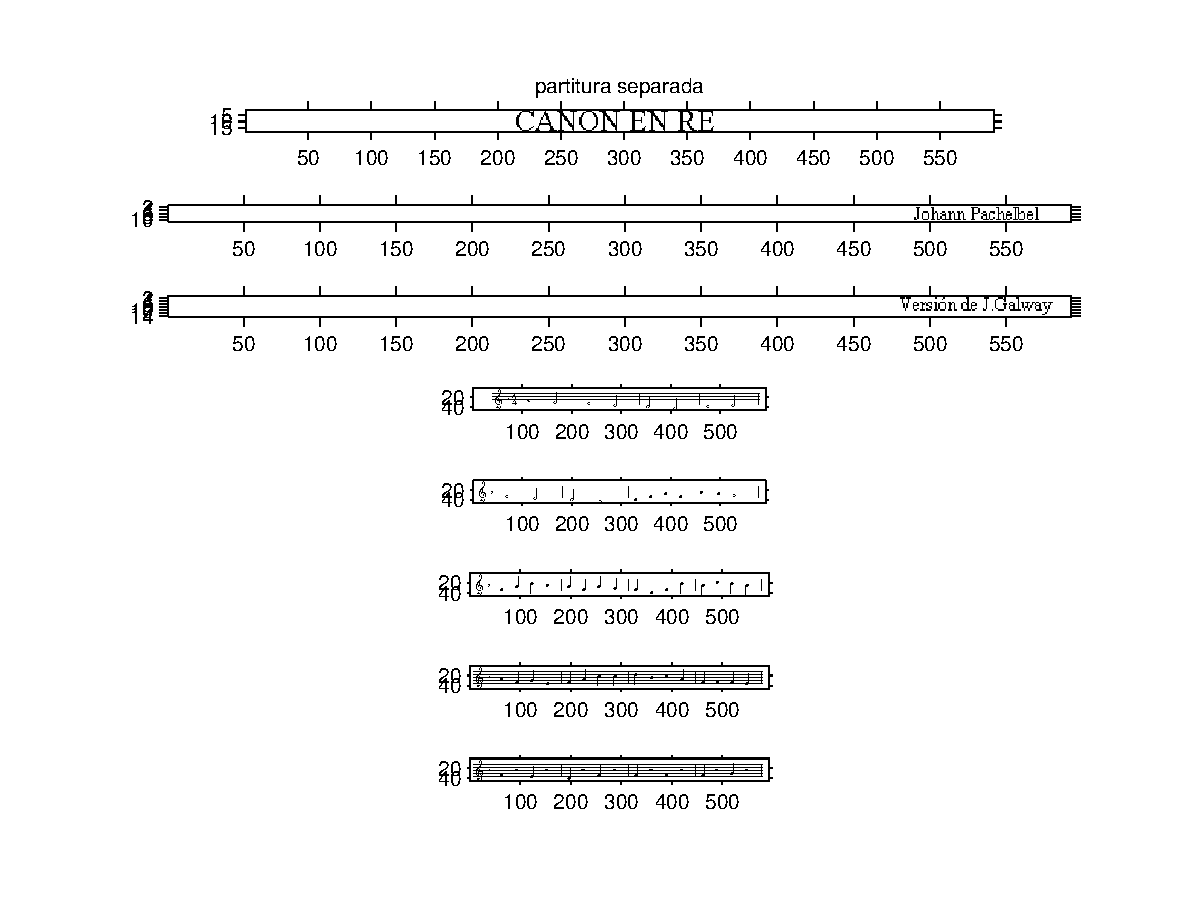
\includegraphics[scale=0.5]{./img1.eps}
  \caption{Resultado de la función corte horizontal}
  \label{fig1}
\end{figure}

Una vez tenemos aislados los pentagramas, separamos los distintos compases. En este caso hay que realizar cortes verticales a lo largo de un solo pentagrama. Las líneas divisorias entre compases son sencillas de localizar porque, una vez el pentagrama está aislado, corresponden a un máximo en el histograma vertical. Sin embargo, no en todas las partituras aparecen al inicio del pentagrama, lo cual nos ha obligado a reducir los requisitos que determinan un corte y luego filtrar las imágenes obtenidas para determinar las que corresponden a compases. Todo esto se realiza mediante \emph{separar\_compases}.


\begin{figure}[h!]
  \centering
    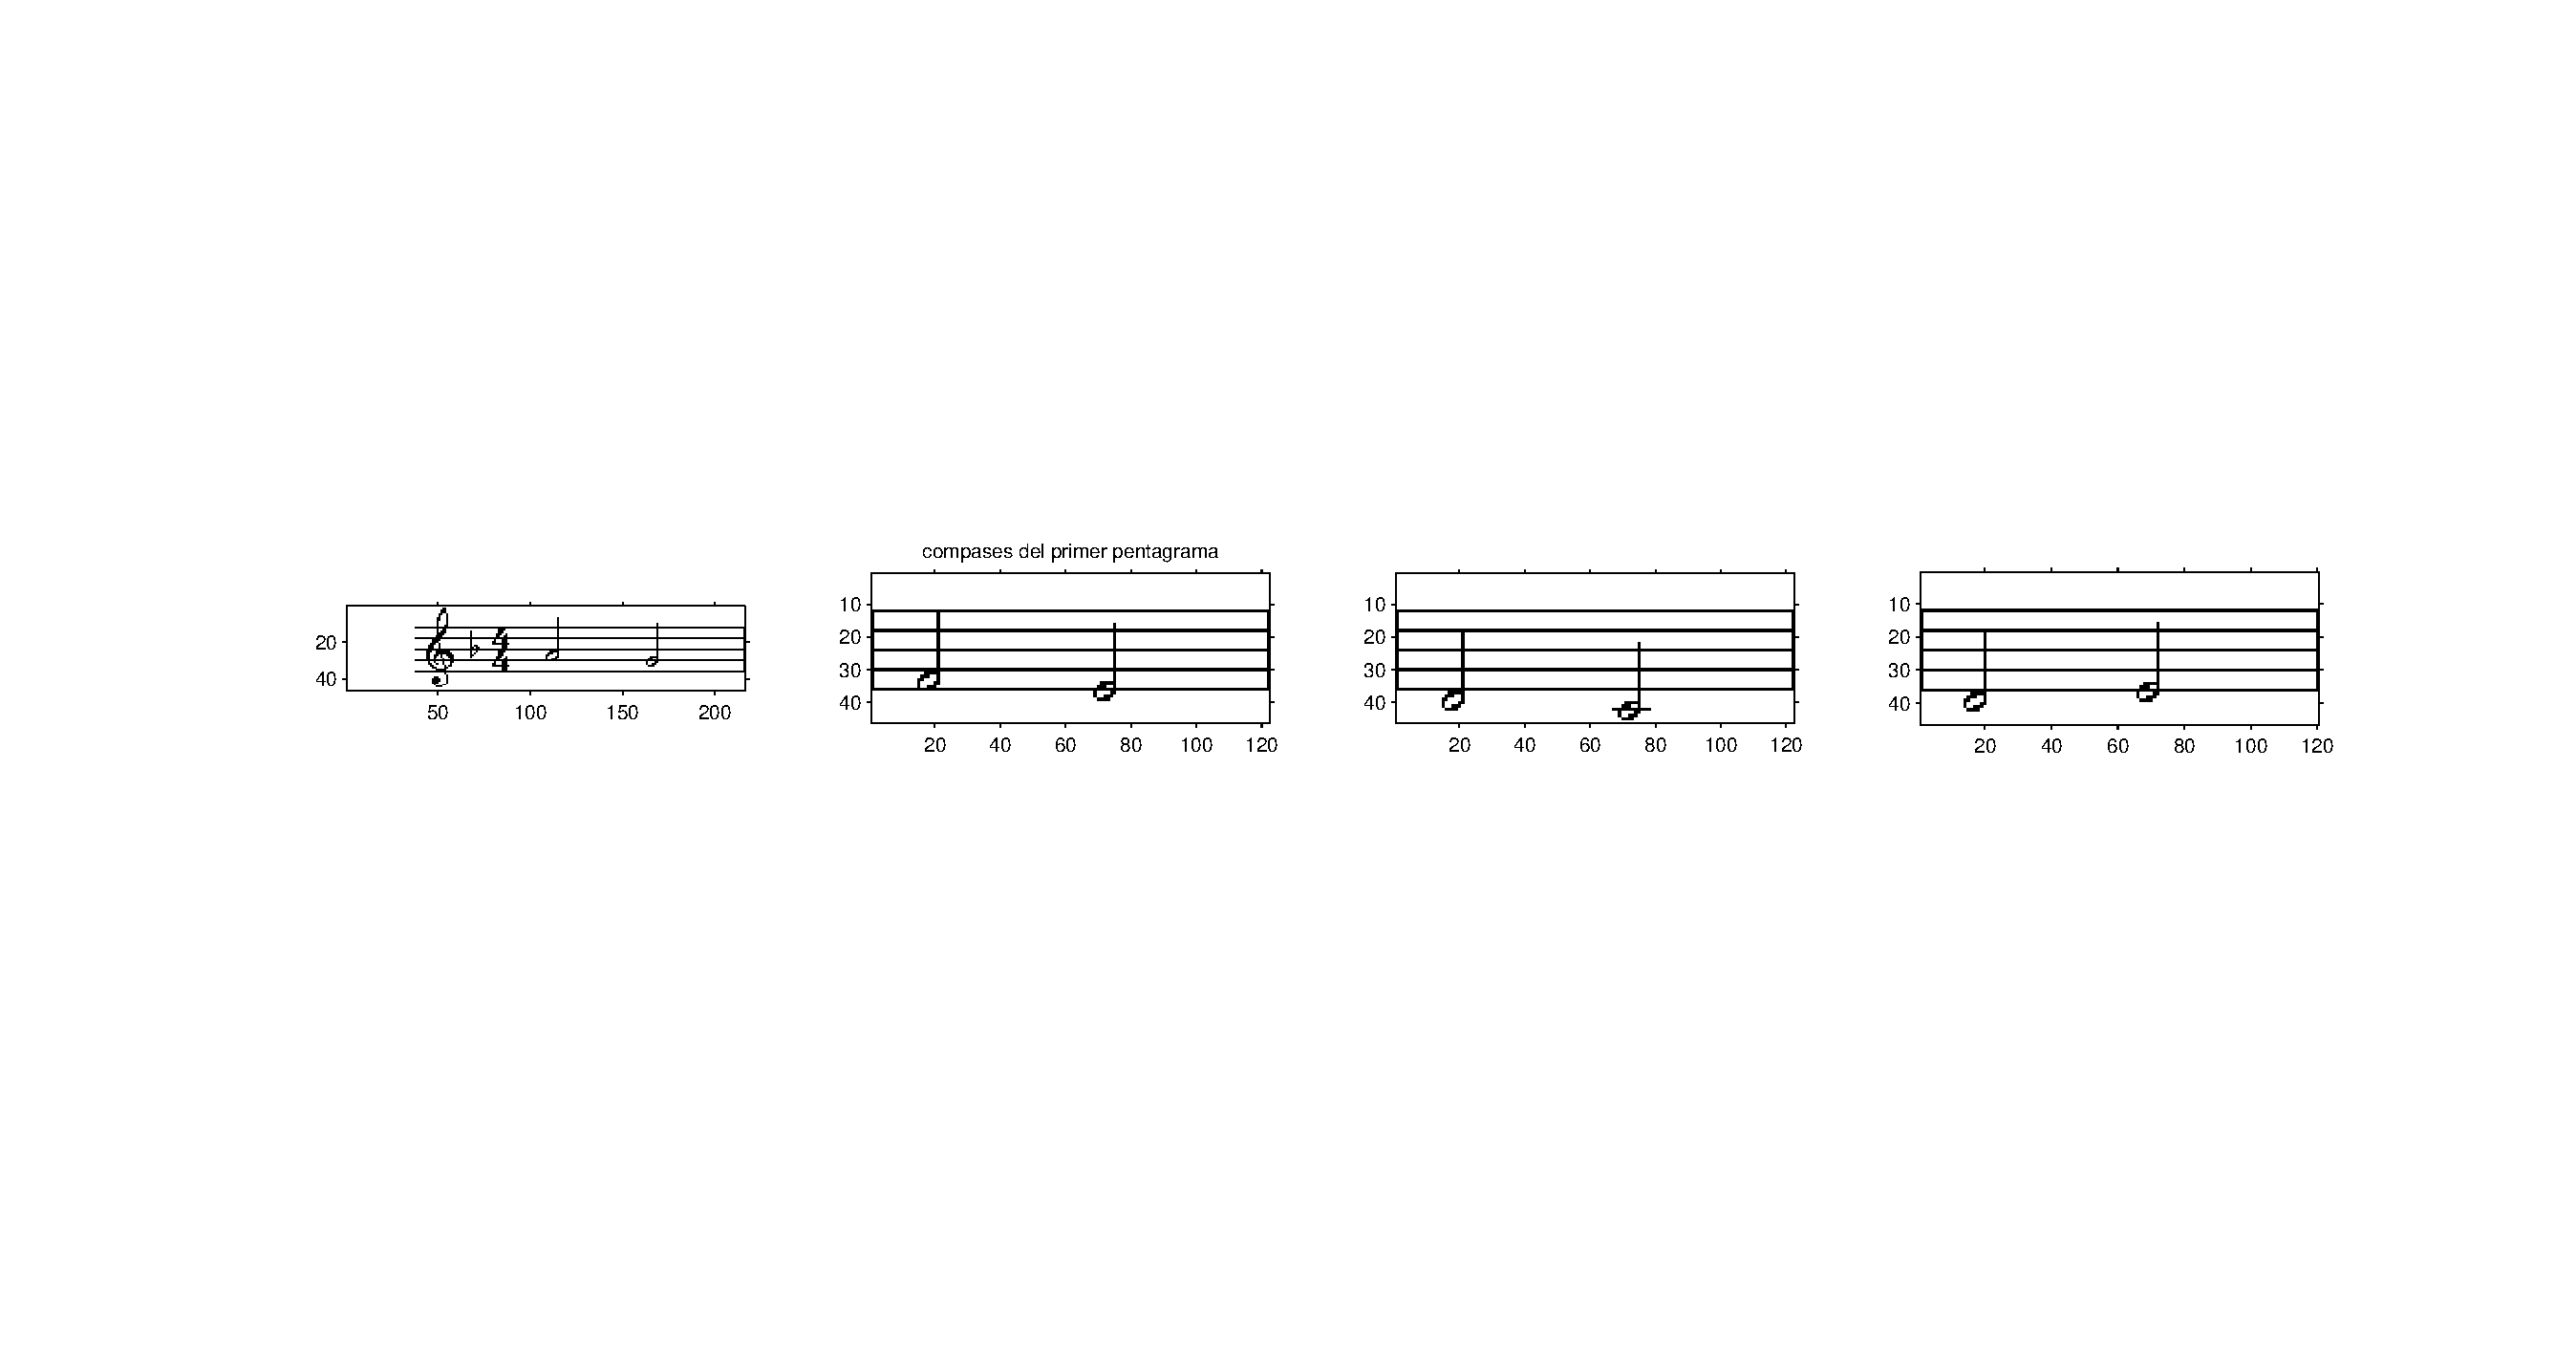
\includegraphics[scale=0.3]{./img2.eps}
  \caption{Resultado de la función separar compases}
  \label{fig1}
\end{figure}


 Por último, para terminar la segmentación queda aislar los elementos que vamos encontrando en cada compás, se vuelve a realizar mediante cortes verticales determinados por \emph{separar\_elementos}.
 

\begin{figure}[h!]
  \centering
    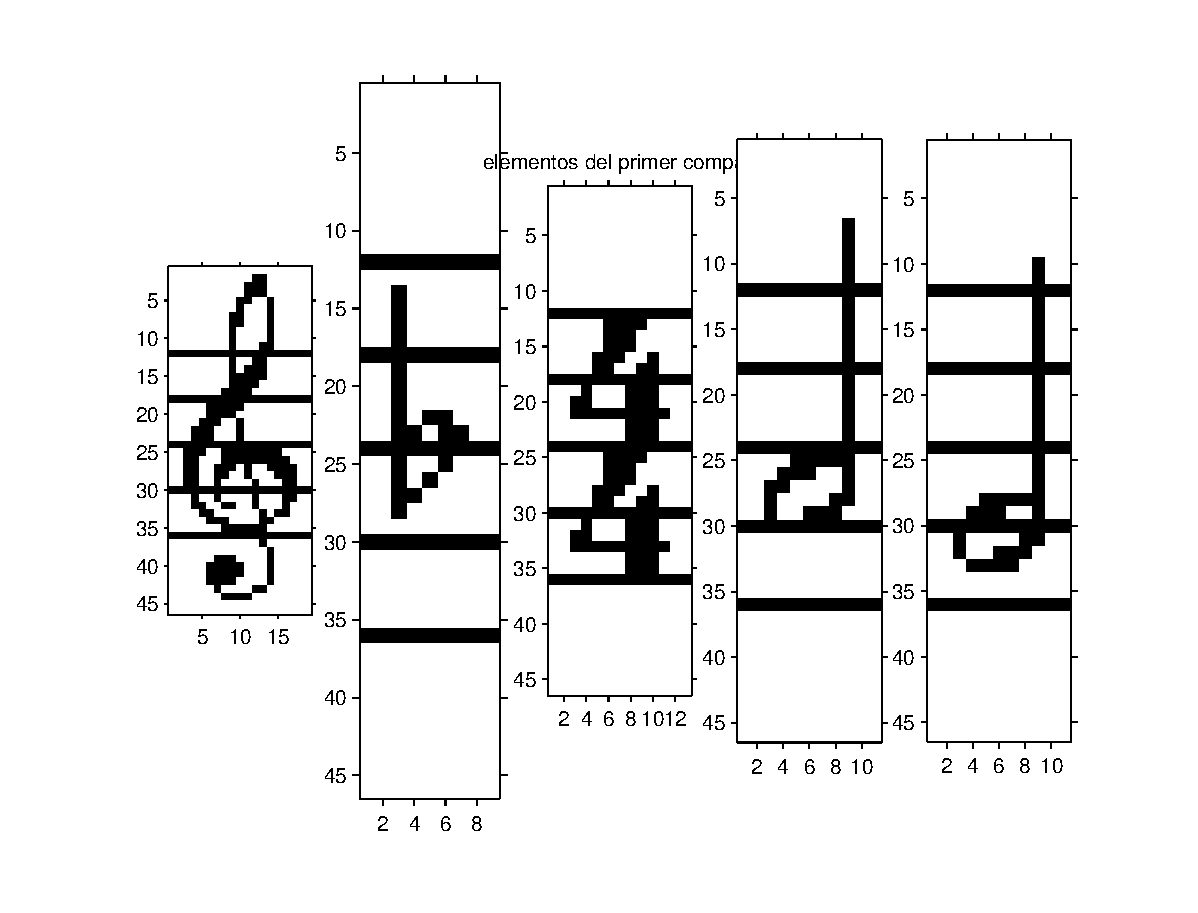
\includegraphics[scale=0.4]{./img3.eps}
  \caption{Resultado de la función separar elementos}
  \label{fig1}
\end{figure}

Realmente, al nivel al que funciona nuestro programa, no es necesaria la separación por compases dado que podrían directamente extraerse uno a uno los elementos de todo el pentagrama. Se ha realizado así pensando en que fuera posible utilizar esa información relativa a la métrica musical en una versión más avanzada del proyecto.

\section{Identificación de elementos}

Al llegar a este paso, tenemos una imagen individual para cada elemento encontrado en el pentagrama. Es necesario ahora identificarlo. Debemos trabajar sobre la imagen para limpiarla, eliminar las lineas del pentagrama y quedarnos solo con la parte que nos interesa. Comparamos la imagen limpia mediante correlación con los elementos de nuestra base de datos, lo cual nos dará el nombre del elemento y su
tipo según el almacenamiento en la base de datos que se explica a continuación.

\begin{figure}[h!]
  \centering
    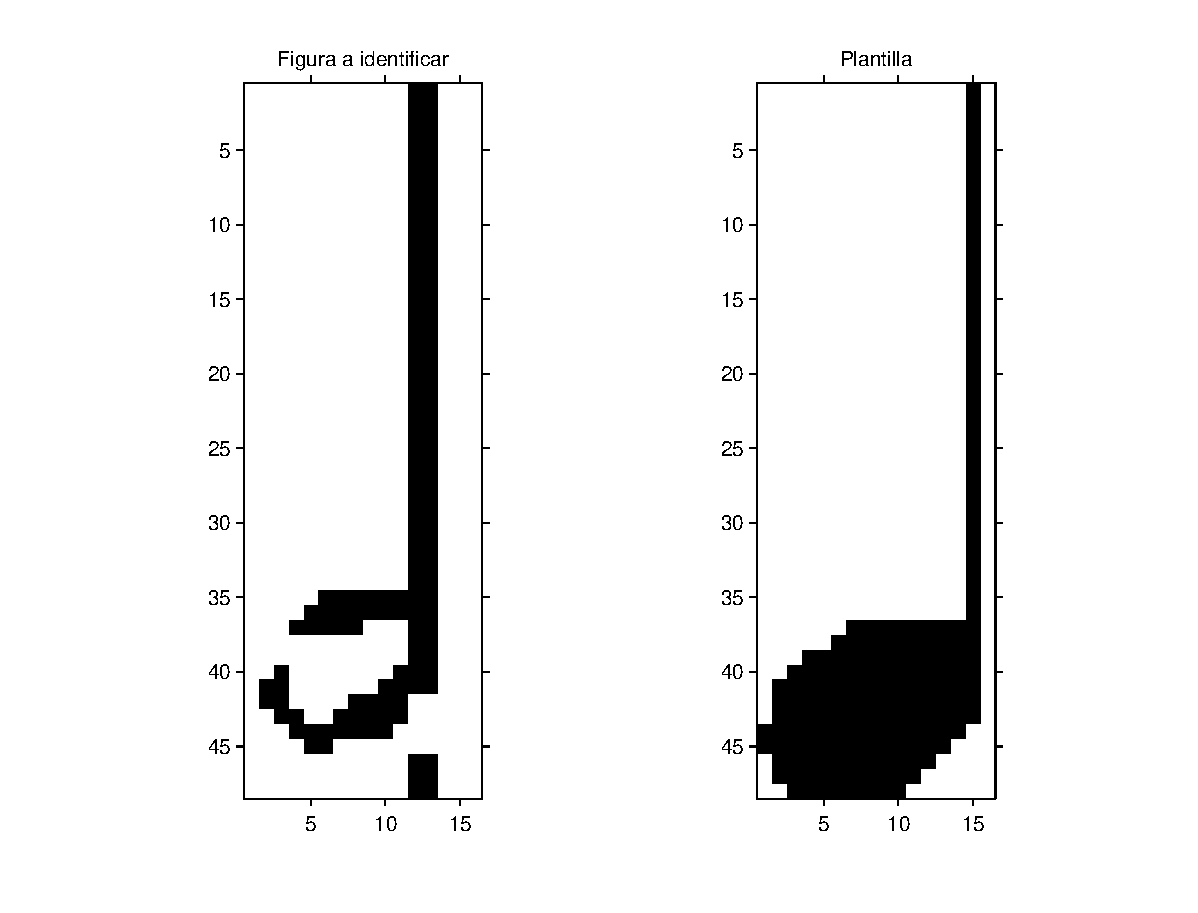
\includegraphics[scale=0.4]{./img4.eps}
  \caption{Ejemplo de comparación entre imágen y máscara}
  \label{fig1}
\end{figure}

\subsection*{Base de datos}

La base de datos es reducida, contiene solo los elementos más básicos que eran los necesarios para trabajar con las imágenes propuestas, pero se ha realizado de forma escalable para que sea sencillo añadir más elementos. Esta organizada en tres tablas que corresponden a notas, silencios u otros. La división de la base de datos esta establecida así para que la gestión de los datos asociados al tipo de figura sea más cómoda. 

\begin{figure}[h!]
  \centering
    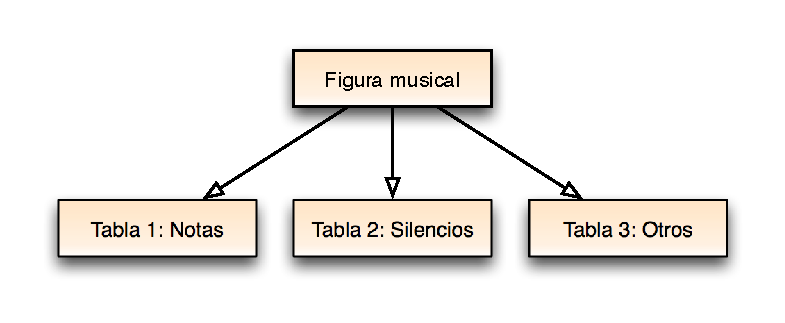
\includegraphics[scale=0.6]{./BD.eps}
  \caption{Jerarquía de la base de datos}
  \label{fig10}
\end{figure}

Para las notas será necesario calcular su altura y de los silencios solo se necesita información relativa a su longitud. El tercer grupo es un poco más amplio, contiene los elementos que aportan información adicional: Claves, velocidad de pentagrama, etc. No se ha utilizado la información que aportan estos elementos, pero el programa es capaz de reconocerlos, por lo que hacer uso de ella no sería complicado más adelante.

A parte de la organización es importante mencionar que se debe ser muy cuidadoso con la elección de las máscaras de la base de datos para que coincidan con las imágenes que se van a extraer de las partituras. Si la máscara no está bien centrada y dimensionada disminuirá mucho el porcentaje de aciertos en las comparaciones.


\section{Altura de la nota}

Si en el paso anterior se detecta que la figura analizada corresponde con una nota, es necesario calcular su altura. Sobre el histograma horizontal, aislamos la cabeza de la nota para saber que posiciones ocupa.

\begin{figure}[h!]
  \centering
    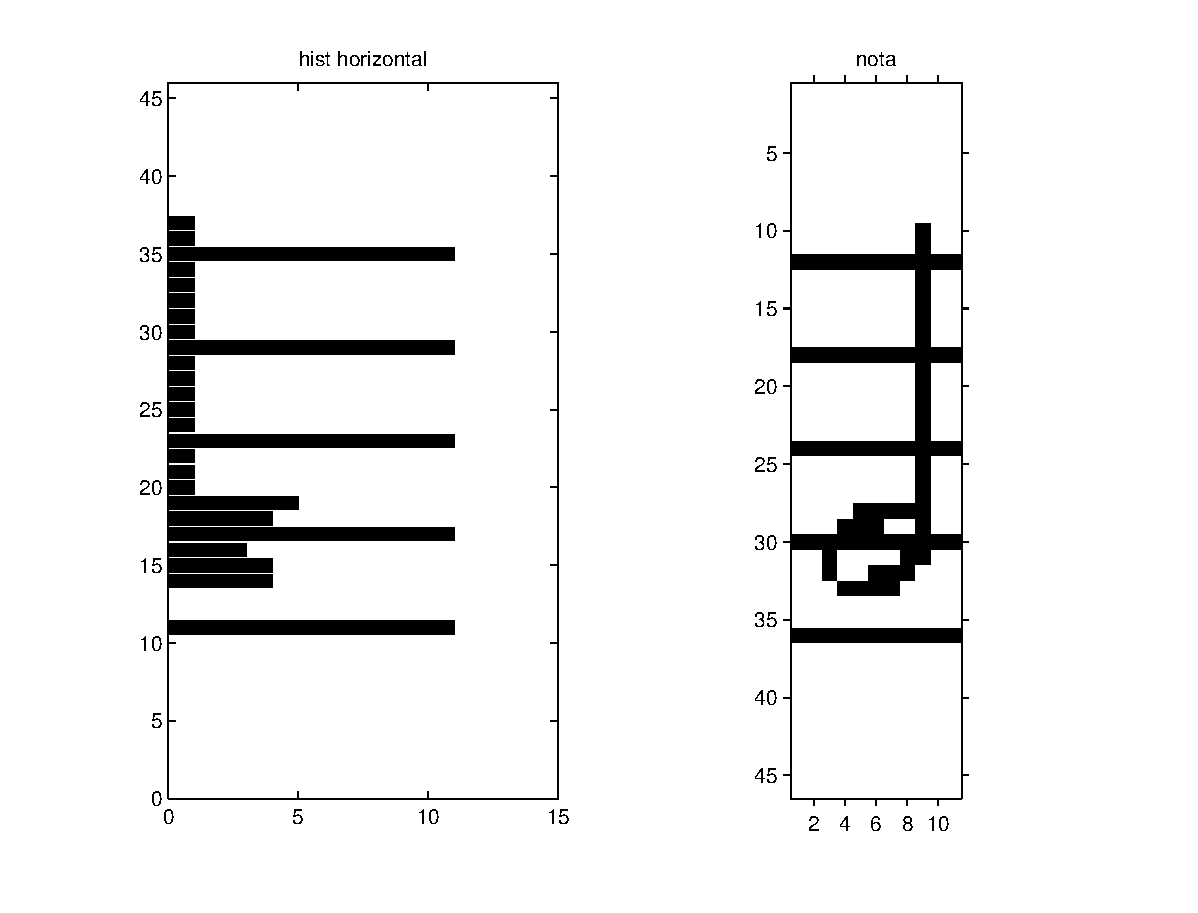
\includegraphics[scale=0.5]{./img5.eps}
  \caption{Nota y su histograma horizontal}
  \label{fig1}
\end{figure}


Dividimos la imagen en intervalos de confianza que cubran las distintas posiciones que puede ocupar una nota sobre el pentagrama. Los intervalos se calculan de forma dinámica en función de la imagen del pentagrama, su altura y el espacio entre líneas. Comprobando en cuál de dichos intervalos cae la media de la cabeza de la nota, obtenemos directamente de qué nota se trata.

\begin{figure}[h!]
  \centering
    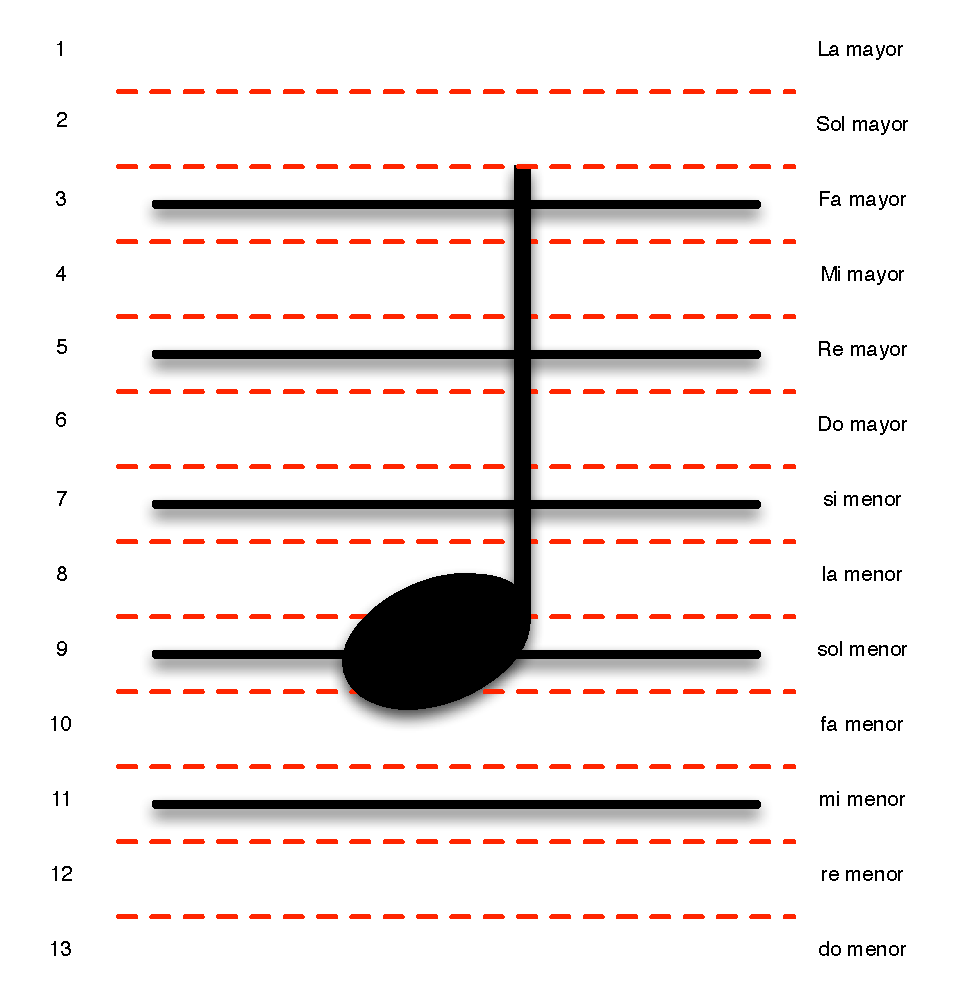
\includegraphics[scale=0.5]{./Espacio_altura.eps}
  \caption{Esquema de la división del espacio}
  \label{fig1}
\end{figure}

El procedimiento esta implementado de forma fija para la clave de sol, cada posición del pentagrama está directamente relacionada con una nota. Sin embargo, como hemos reconocido previamente la clave correspondiente al pentagrama, es sencillo implementar una mejora que utilice la información correspondiente a la clave y calcule la altura de la nota en consecuencia. No se ha realizado por considerar que era una inversión grande de tiempo en algo poco relacionado con el tratamiento de la imagen en sí. Nótese también que la nota se reconoce como un valor numérico antes de asignarle un nombre de tipo texto, esto permite crear una notación comprensible para la máquina si en lugar de pasar a texto la partitura, se pretende reproducirla. Esto facilita la posibilidad de obtener distintas salidas sin tener que modificar el método de lectura.

El método implementado funciona tan solo con notas simples, pero podría ampliarse para reconocer acordes (dos o más notas distintas tocadas a la vez) haciendo una comprobación de la longitud de las posiciones que ocupa la cabeza de la nota (en caso de que estén muy juntas) o si se encuentra un número de intervalos de posiciones de cabeza mayor que uno (en caso de que estén separadas).

\section{Proceso}

Para leer la partitura se procede en primer lugar por pentagramas, para cada pentagrama, se obtienen todos los compases que lo forman, y para cada compás, todos sus elementos. De esta forma, cuando se ha acabado con un pentagrama completo, se procede al siguiente, y así sucesivamente hasta haber finalizado la partitura. 

La información relativa a cada elemento se va almacenando en forma de texto en una variable partitura en la que se introduce un salto de línea cada pentagrama para que sea más cómoda la visualización.

\section{Conclusiones}

El proyecto de reconocer partituras musicales no ha resultado ser excesivamente complejo conceptualmente sin embargo, durante su desarrollo, han surgido una cantidad considerable de pequeños problemas y casos particulares que nos han impedido desarrollar algunas cosas con profundidad. Cabe mencionar por ejemplo la precisión que ha sido necesaria en el aislamiento de la figura de la nota blanca para que la correlación con su modelo fuera la correcta, que en un principio devolvía el resultado negra en la mayoría de los casos.

También supuso un problema reconocer los silencios de blanca y de redonda, cuya forma es la misma y dependen de su posición sobre el pentagrama, lo cual nos ha obligado a hacer una comprobación extra en el caso de que la correlación devuelva alguno de estos silencios.

Las máscaras nos dieron problemas en muchos casos. Hemos llegado a la conclusión de que es imprescindible evitar que la imagen sufra una reducción de tamaño al redimensionarse para comparar con la máscara. La máscara debe ser siempre de mayor tamaño que las imágenes extraídas para comparación. Al trabajar con máscaras es importante conseguir el modelo más genérico posible, optimizar un resultado puede redundar en estropear otros, como nos ha pasado finalmente con las notas negras, que a veces se reconocen como blancas. Cabe la posibilidad de mejorar el resultado utilizando una base de datos más amplia o entrenando el sistema.

\end{document}